\documentclass[11pt,a4paper]{article}
\usepackage[utf8]{inputenc}
\usepackage[T1]{fontenc}
\usepackage[spanish]{babel}
\usepackage{geometry}
\geometry{margin=2cm}
\usepackage{hyperref}
\usepackage{xcolor}
\usepackage{booktabs}
\usepackage{longtable}
\usepackage{enumitem}
\usepackage{graphicx}
\usepackage{titlesec}
\usepackage{fancyhdr}
\usepackage{float}
\usepackage{subcaption}
\usepackage{wrapfig}

\graphicspath{
  {../refactorizacion-variable/diagrams/}
  {../refactorizacion-node/diagrams/}
  {../analisis-probnet/diagrams/}
  {../refactorizacion-discrete-potential-operations/}
  {../rediseno-potenciales/diagrams/}
  {../refactorizacion-excepciones-previo/}
  {../refactorizacion-excepciones-posterior/}
  {../heuristic/}
}

\definecolor{bugfix}{RGB}{220,50,50}
\definecolor{refactor}{RGB}{50,120,200}
\definecolor{test}{RGB}{50,160,50}
\definecolor{docs}{RGB}{140,100,180}
\definecolor{cleanup}{RGB}{120,120,120}
\definecolor{problem}{RGB}{180,40,40}
\definecolor{solution}{RGB}{40,120,40}

\pagestyle{fancy}
\fancyhead[L]{OpenMarkov --- Resumen de cambios}
\fancyhead[R]{28 mar -- 7 abr 2026}
\fancyfoot[C]{\thepage}

\title{\textbf{Resumen de cambios en OpenMarkov}\\[0.3em]
\large Período: 28 de marzo -- 7 de abril de 2026}
\author{Manuel Arias --- CISIAD, UNED}
\date{7 de abril de 2026}

\begin{document}
\maketitle
\tableofcontents
\newpage

%==============================================================================
\section{Visión general}
%==============================================================================

En los últimos 10 días se han realizado \textbf{152 commits} distribuidos en \textbf{19 módulos}.
El trabajo se ha organizado en seis ejes principales:

\begin{enumerate}[leftmargin=2cm,label=\textbf{Eje \arabic*:}]
  \item \textbf{Refactorización de clases core} --- Extracción de responsabilidades de las clases dios (\texttt{Variable}, \texttt{Node}, \texttt{ProbNet}, \texttt{DiscretePotentialOperations}) y rediseño de la jerarquía de potenciales.
  \item \textbf{Corrección de bugs} --- 11 issues resueltos (\#456, \#472, \#486, \#496, \#497, \#504, \#506, \#520, \#532, \#562, separación de conjuntos en PC).
  \item \textbf{Calidad de código} --- 470 variables marcadas \texttt{final}, 178 imports no usados eliminados, 502 tags Javadoc añadidos, métodos redundantes eliminados.
  \item \textbf{Tests} --- Nuevos tests de invariantes algebraicos, tests de regresión de \texttt{tableProject}, tests de \texttt{GTablePotential}, tests unitarios de \texttt{Criterion}, \texttt{Finding} y aritmética de \texttt{TablePotential}.
  \item \textbf{Rediseño de potenciales} --- Reparentado de \texttt{GTablePotential}, interfaces de capacidad, encapsulación de \texttt{TablePotential.values}.
  \item \textbf{Documentación técnica} --- 12 documentos LaTeX con 51 diagramas UML PlantUML describiendo cada refactorización.
\end{enumerate}

\bigskip
\noindent\textbf{Distribución de commits por módulo:}

\begin{center}
\begin{tabular}{lr}
\toprule
\textbf{Módulo} & \textbf{Commits} \\
\midrule
org.openmarkov.core         & 44 \\
org.openmarkov.inference    & 19 \\
org.openmarkov.gui          & 17 \\
org.openmarkov.io           & 11 \\
org.openmarkov.learning.algorithm & 9 \\
org.openmarkov.integrationtests   & 9 \\
org.openmarkov (POM/docs)   & 8 \\
org.openmarkov.learning.core & 7 \\
org.openmarkov.learning.gui  & 5 \\
Otros 10 módulos (1--4 c/u) & 23 \\
\midrule
\textbf{Total}              & \textbf{152} \\
\bottomrule
\end{tabular}
\end{center}

%==============================================================================
\section{Refactorización de Variable}
\label{sec:variable}
%==============================================================================

\noindent\textit{Documento completo:} \texttt{docs/refactorizacion-variable/refactorizacion-variable.tex}

\subsection{Problema}

La clase \texttt{Variable} (986 líneas) mezclaba dos responsabilidades fundamentalmente distintas: ser un \textbf{objeto de dominio} (nombre, tipo, estados) y contener \textbf{lógica de edición del grafo} que dependía de \texttt{Node}, \texttt{ProbNet} y \texttt{Link}. Esto causaba:

\begin{itemize}
  \item \textcolor{problem}{\textbf{Dependencia circular conceptual:}} \texttt{Variable} (dominio) dependía de \texttt{Node} (grafo), pero \texttt{Node} contenía una \texttt{Variable}. Modificar la lógica de edición de estados requería entender y tocar la clase de dominio.
  \item \textcolor{problem}{\textbf{Sincronización frágil:}} Los campos \texttt{name}, \texttt{baseName} y \texttt{timeSlice} se sincronizaban en 3 puntos distintos con side-effects: llamar a \texttt{setBaseName()} después de \texttt{setName()} podía dejar el estado interno inconsistente.
  \item \textcolor{problem}{\textbf{Ordenación no determinista:}} \texttt{compareTo()} usaba \texttt{hashCode()}, lo que producía un orden no reproducible entre ejecuciones de la JVM.
\end{itemize}

\begin{figure}[H]
  \centering
  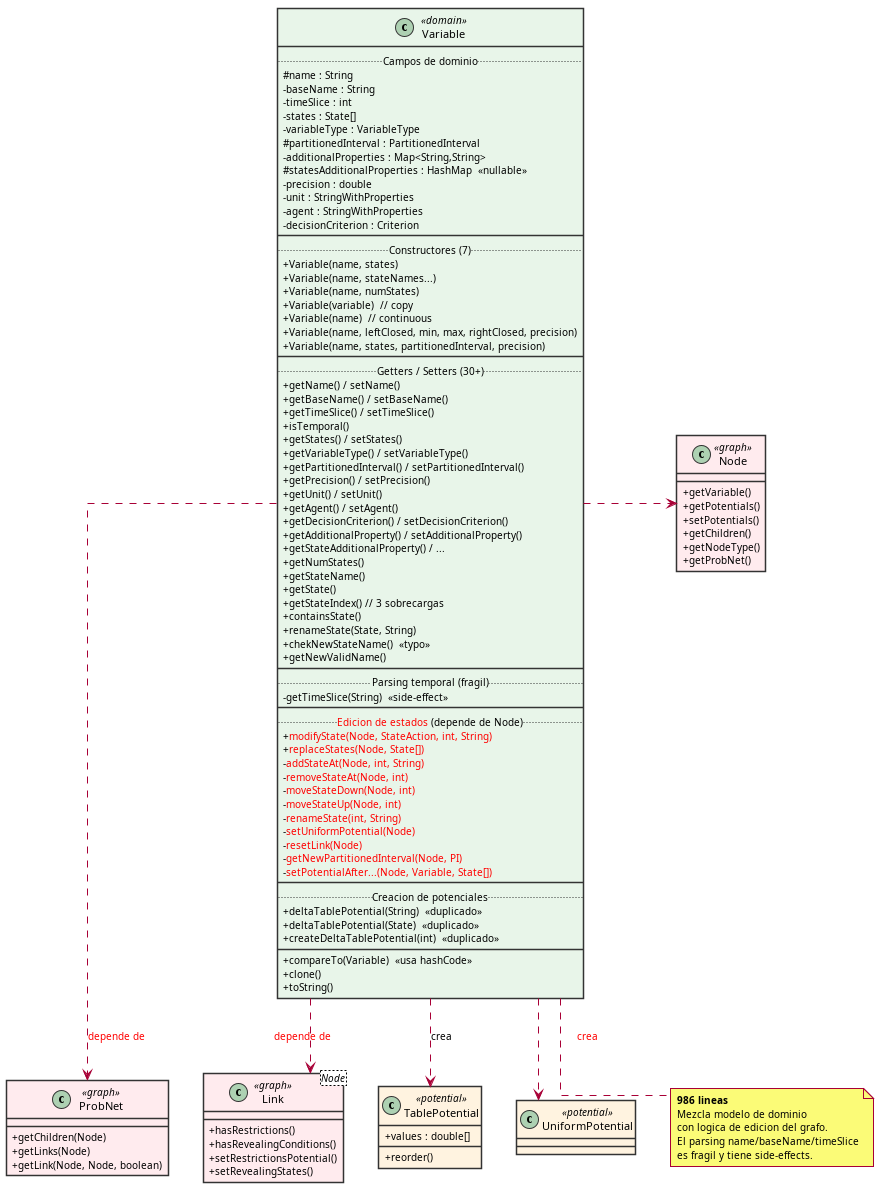
\includegraphics[width=0.9\textwidth]{variable-antes}
  \caption{Variable antes de la refactorización: 986 líneas con 12 métodos de edición de estados (en rojo) que dependen de \texttt{Node}, \texttt{ProbNet} y \texttt{Link}. Nótese la anotación \texttt{<<typo>>} en \texttt{chekNewStateName()} y \texttt{<<usa hashCode>>} en \texttt{compareTo()}.}
  \label{fig:var-antes}
\end{figure}

\subsection{Solución}

Extracción de los 12 métodos de edición de estados a una clase estática de utilidad \texttt{VariableStateOperations}, y consolidación de la sincronización temporal en dos métodos idempotentes.

\begin{figure}[H]
  \centering
  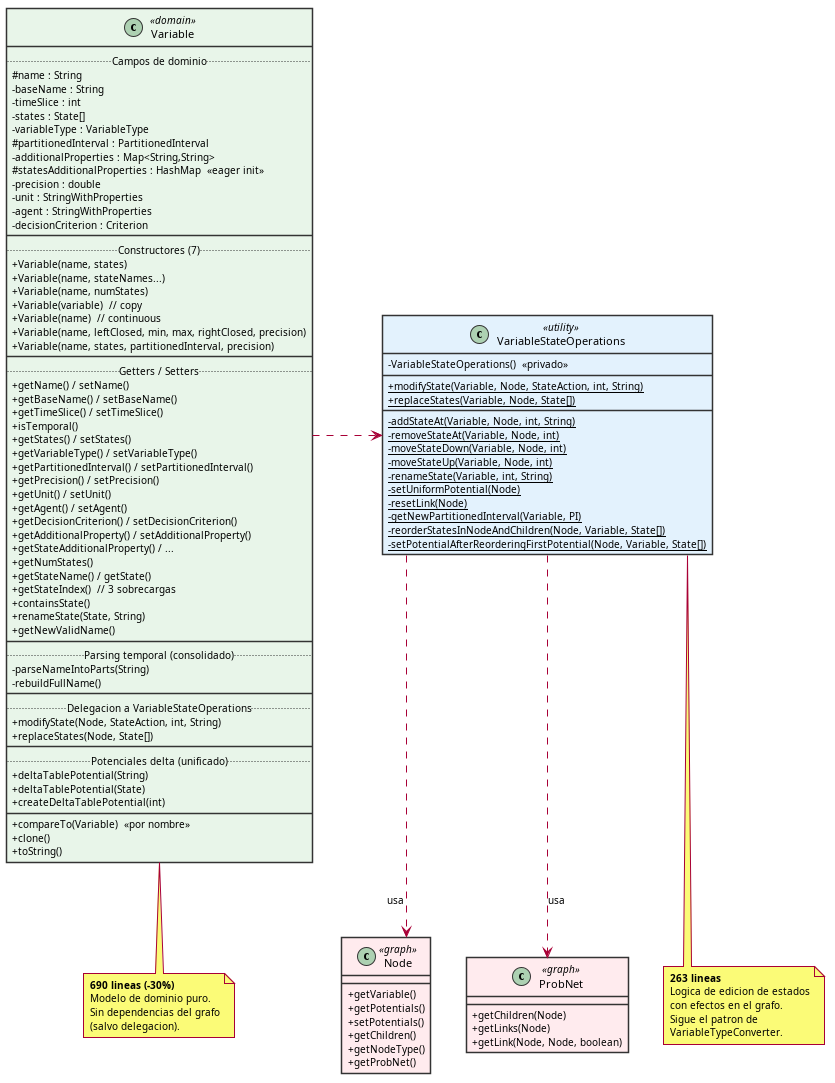
\includegraphics[width=0.95\textwidth]{variable-despues}
  \caption{Variable después: 690 líneas (--30\%). La lógica de edición de estados vive en \texttt{VariableStateOperations} (263 líneas). \texttt{Variable} queda como modelo de dominio puro con delegación. El parsing temporal se consolida en \texttt{parseNameIntoParts()} / \texttt{rebuildFullName()}.}
  \label{fig:var-despues}
\end{figure}

\subsection{Por qué aporta}

\begin{enumerate}
  \item \textbf{Testabilidad:} Los métodos de edición de estados ahora son estáticos y se pueden testear aisladamente sin construir un \texttt{Variable} completo. Los tests pasaron de 28 a 99.
  \item \textbf{Mantenibilidad:} Modificar la lógica de edición ya no requiere tocar la clase de dominio. Un cambio en cómo se recalculan los potenciales tras añadir un estado solo afecta a \texttt{VariableStateOperations}.
  \item \textbf{Determinismo:} El \texttt{compareTo()} por nombre alfabético es estable y reproducible, eliminando errores intermitentes en estructuras ordenadas (\texttt{TreeSet}, \texttt{SortedMap}).
  \item \textbf{Robustez temporal:} La consolidación de \texttt{name}/\texttt{baseName}/\texttt{timeSlice} elimina la clase de bugs donde ``\texttt{X [3]}'' se parseaba como baseName=``\texttt{X}'' pero luego \texttt{setBaseName(``Y'')} no actualizaba \texttt{name}.
\end{enumerate}

\begin{figure}[H]
  \centering
  \begin{subfigure}[b]{0.48\textwidth}
    \centering
    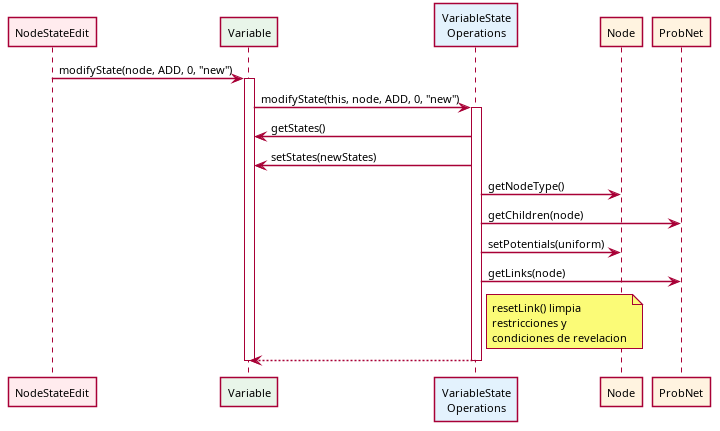
\includegraphics[width=\textwidth]{flujo-delegacion}
    \caption{Flujo de delegación: el edit llama a \texttt{Variable}, que delega a \texttt{VariableStateOperations}, que opera sobre \texttt{Node} y \texttt{ProbNet}.}
  \end{subfigure}
  \hfill
  \begin{subfigure}[b]{0.48\textwidth}
    \centering
    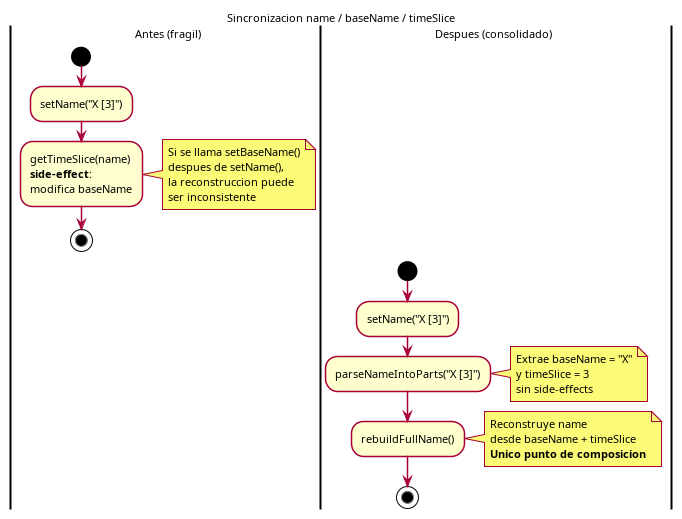
\includegraphics[width=\textwidth]{name-sync}
    \caption{Antes: sincronización frágil con side-effects. Después: dos métodos idempotentes sin side-effects.}
  \end{subfigure}
  \caption{Diagramas de secuencia y actividad de la refactorización de Variable.}
\end{figure}

%==============================================================================
\section{Refactorización de Node}
\label{sec:node}
%==============================================================================

\noindent\textit{Documento completo:} \texttt{docs/refactorizacion-node/refactorizacion-node.tex}

\subsection{Problema}

La clase \texttt{Node} (1.037 líneas) tenía \textbf{6 razones para cambiar}: identidad del nodo, CRUD de potenciales, delegación al grafo, metadatos, presentación visual, y 308 líneas de lógica compleja de transformación (absorción, conversión de tipos, funciones de utilidad). Cada una de estas lógicas complejas era invocada por exactamente un caller externo, lo que hacía de \texttt{Node} un ``vertedero'' de funcionalidad.

\begin{figure}[H]
  \centering
  
\includegraphics[width=1.0\textwidth]{before}
  \caption{Node antes: 1.037 líneas con 5 bloques de lógica de transformación (en negrita) que no pertenecen a la identidad del nodo. Cada bloque es invocado por un único caller (amarillo).}
  \label{fig:node-antes}
\end{figure}

\subsection{Solución}

Aplicación del patrón \textbf{Extract Class} en 5 fases, extrayendo cada bloque a la clase que lo necesita o a una clase de utilidad estática enfocada:

\begin{figure}[H]
  \centering
  
\includegraphics[width=\textwidth]{after}
  \caption{Node después: 670 líneas (--35\%). La lógica de transformación se ha extraído a 3 clases nuevas (verde) y 1 clase existente (gris). Cada caller ahora invoca directamente la clase especializada.}
  \label{fig:node-despues}
\end{figure}

\subsection{Por qué aporta}

\begin{figure}[H]
  \centering
  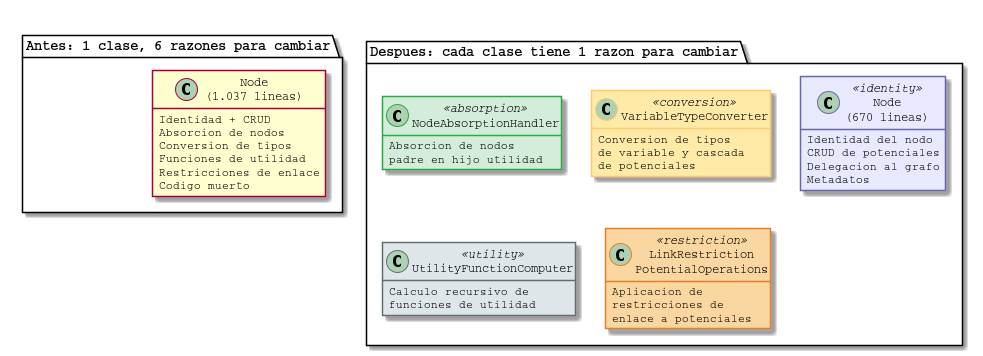
\includegraphics[width=\textwidth]{srp}
  \caption{Aplicación del Principio de Responsabilidad Única: de 1 clase con 6 razones para cambiar a 5 clases con 1 razón cada una.}
  \label{fig:node-srp}
\end{figure}

\begin{enumerate}
  \item \textbf{SRP (Single Responsibility Principle):} Cada clase tiene ahora una única razón para cambiar. Un bug en la absorción de nodos solo requiere modificar \texttt{NodeAbsorptionHandler}, sin riesgo de afectar al CRUD de potenciales ni a la presentación visual.
  \item \textbf{Cohesión:} \texttt{absorbNodeConsistently()} (78 líneas) operaba sobre potenciales, arcos y variables --- una operación completa de alto nivel que no tiene relación con la identidad de un nodo. Ahora vive donde le corresponde: en \texttt{NodeAbsorptionHandler}, junto a \texttt{AbsorbNodeEdit} que es su único usuario.
  \item \textbf{Descubribilidad:} Antes, un desarrollador que buscara ``absorción de nodos'' lo encontraría enterrado a la mitad de una clase de 1.037 líneas. Ahora tiene una clase dedicada cuyo nombre anuncia su propósito.
  \item \textbf{Sin rotura de API:} Los callers existentes (\texttt{AbsorbNodeEdit}, \texttt{VariableTypeEdit}, etc.) fueron modificados para usar las clases extraídas, pero la interfaz pública de \texttt{Node} se mantuvo intacta para el resto del sistema.
\end{enumerate}

%==============================================================================
\section{Análisis de ProbNet y extracción de responsabilidades}
\label{sec:probnet}
%==============================================================================

\noindent\textit{Documento completo:} \texttt{docs/analisis-probnet/analisis-probnet.tex}

\subsection{Problema}

\texttt{ProbNet} es la clase más crítica de OpenMarkov: 1.440 líneas, 80+ métodos públicos, referenciada por 490 ficheros. Es un ejemplo de libro de texto del antipatrón \textbf{God Class}: concentra nodos, links, variables, potenciales, constraints, agentes, clasificación de redes, y metadatos de I/O en una sola clase.

\begin{figure}[H]
  \centering
  
\includegraphics[width=0.85\textwidth]{probnet-actual}
  \caption{ProbNet actual: 1.440 líneas con 80+ métodos. Los colores indican responsabilidades: verde=nodos/links/variables, naranja=potenciales, azul=constraints, rojo=clasificación, púrpura=agentes. Los campos \texttt{reader}/\texttt{writer} (etiquetados SRP) acoplan el modelo de dominio al I/O.}
  \label{fig:probnet-actual}
\end{figure}

El análisis identificó 4 bugs confirmados y 7 code smells:

\begin{figure}[H]
  \centering
  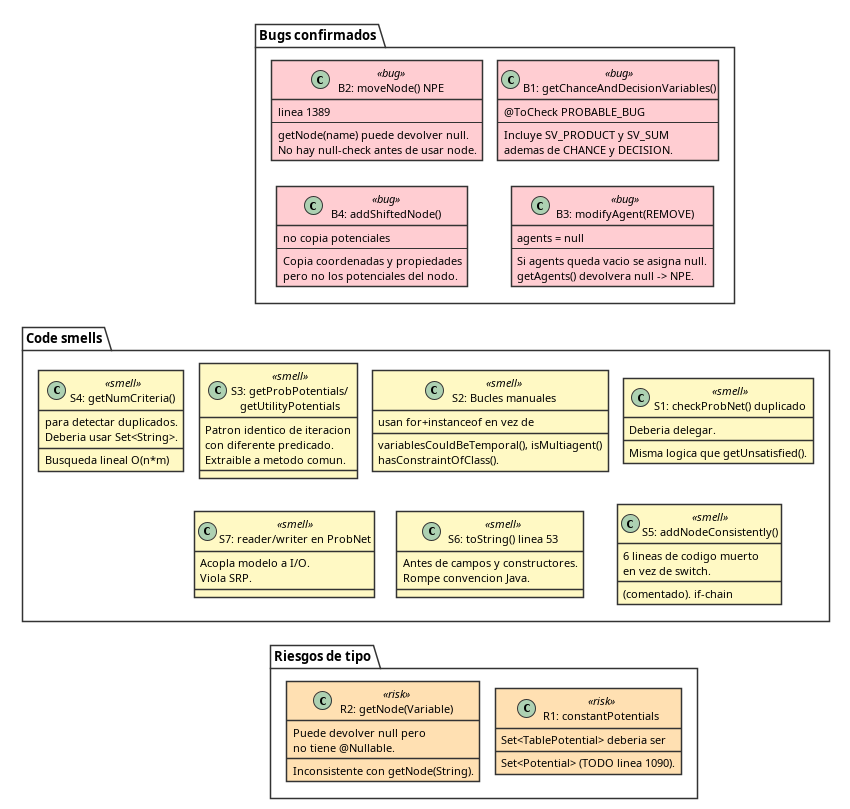
\includegraphics[width=\textwidth]{bugs-detectados}
  \caption{Bugs detectados en ProbNet (rojo), code smells (amarillo) y riesgos de tipo (naranja). B2 (\texttt{moveNode()} NPE) y B3 (\texttt{modifyAgent(REMOVE)} dejando \texttt{null}) son errores de null-safety; B4 (\texttt{addShiftedNode()}) pierde información; S7 (reader/writer) viola SRP y DIP.}
  \label{fig:probnet-bugs}
\end{figure}

\subsection{Solución (implementada parcialmente)}

Se extrajeron 3 clases de utilidad, reduciendo ProbNet en $\sim$340 líneas:

\begin{figure}[H]
  \centering
  
\includegraphics[width=0.85\textwidth]{probnet-propuesta}
  \caption{ProbNet propuesta ($\sim$1.100 líneas, --24\%): las responsabilidades de clasificación, gestión de agentes y consultas de potenciales se han extraído a clases estáticas dedicadas (azul). El modelo queda como grafo + constraints + metadatos.}
  \label{fig:probnet-propuesta}
\end{figure}

\subsection{Por qué aporta}

\begin{enumerate}
  \item \textbf{Reducción del radio de impacto:} Con 490 ficheros referenciando \texttt{ProbNet}, cualquier cambio tiene un potencial de propagación enorme. Extraer responsabilidades reduce el número de razones por las que hay que modificar la clase central.
  \item \textbf{Testabilidad:} Los 6 métodos de clasificación (antes con 0\% de cobertura) ahora son estáticos en \texttt{ProbNetClassifier} y se pueden testear sin construir toda la infraestructura de \texttt{ProbNet}.
  \item \textbf{Corrección de bugs:} La gestión de agentes (S3, con bug de \texttt{null}) fue extraída a \texttt{ProbNetAgentManager}, donde el bug fue visible y corregible sin riesgo de afectar nodos o potenciales.
  \item \textbf{Desacoplamiento I/O:} La propuesta de eliminar \texttt{reader}/\texttt{writer} de \texttt{ProbNet} (fase 6, pendiente) eliminaría la violación del Dependency Inversion Principle: un modelo de dominio no debería depender de su mecanismo de persistencia.
\end{enumerate}

%==============================================================================
\section{Refactorización de DiscretePotentialOperations}
\label{sec:dpo}
%==============================================================================

\noindent\textit{Documento completo:} \texttt{docs/refactorizacion-discrete-potential-operations/}

\subsection{Problema}

\texttt{DiscretePotentialOperations} (2.175 líneas) era la segunda clase más grande del core: 28 métodos públicos estáticos y $\sim$15 privados, cubriendo aritmética, eliminación, maximización, fusión, transformación y factoría de potenciales. El problema no era solo el tamaño, sino que un bug en \texttt{normalize()} podía estar a 50 líneas de \texttt{multiplyAndMaximize()}, en un fichero donde era imposible navegar sin buscar.

\begin{figure}[H]
  \centering
  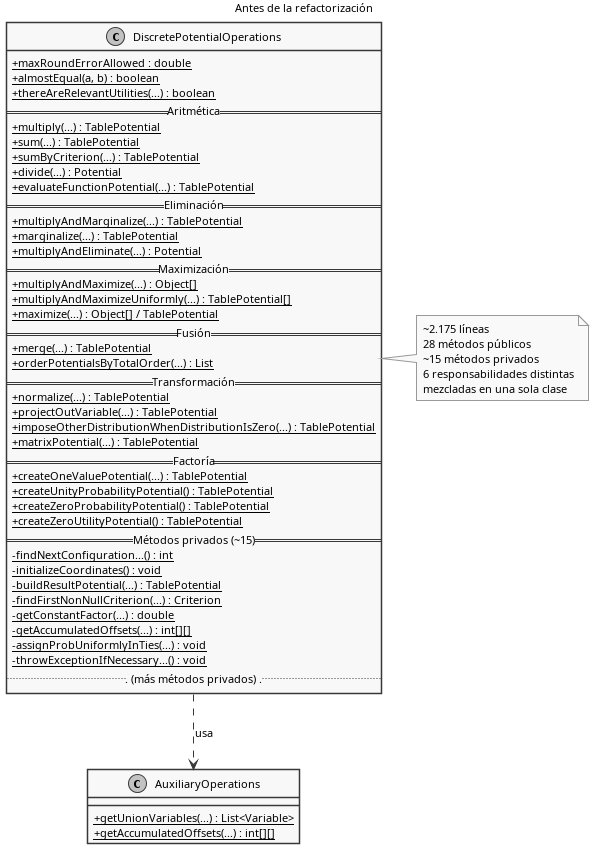
\includegraphics[width=0.55\textwidth]{antes}
  \caption{Antes: una clase monolítica de 2.175 líneas con 6 responsabilidades mezcladas. Los métodos privados ($\sim$15) están compartidos sin criterio claro.}
  \label{fig:dpo-antes}
\end{figure}

\subsection{Solución}

Aplicación del patrón \textbf{Facade}: \texttt{DiscretePotentialOperations} se mantiene como API pública ($\sim$460 líneas de delegación pura), pero la implementación se distribuye en 6 clases package-scoped organizadas por responsabilidad:

\begin{figure}[H]
  \centering
  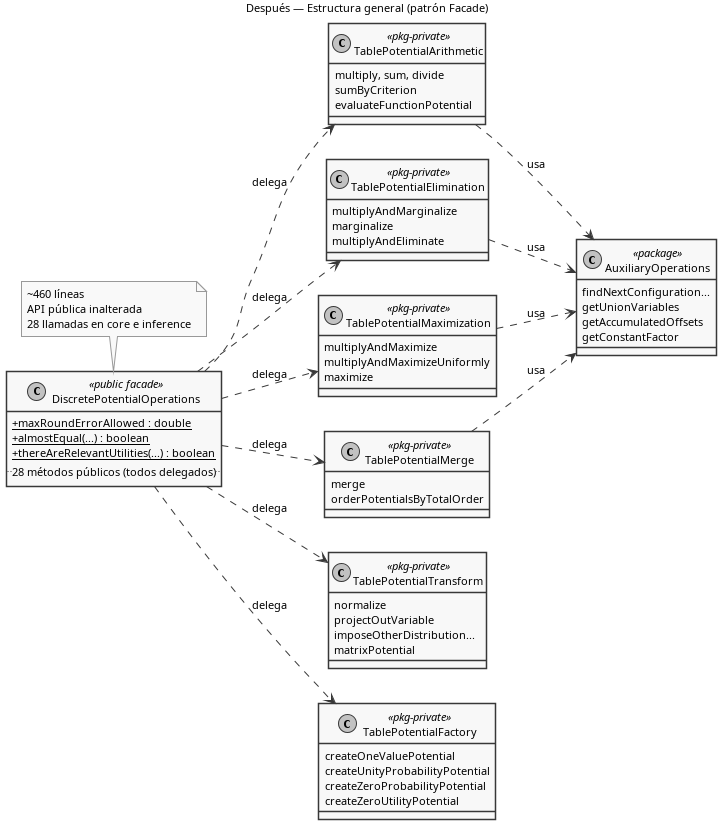
\includegraphics[width=0.85\textwidth]{despues-estructura}
  \caption{Después: Facade pública inalterada + 6 clases de implementación package-scoped. Cada clase contiene los métodos de una sola responsabilidad y sus helpers privados asociados.}
  \label{fig:dpo-estructura}
\end{figure}

\begin{figure}[H]
  \centering
  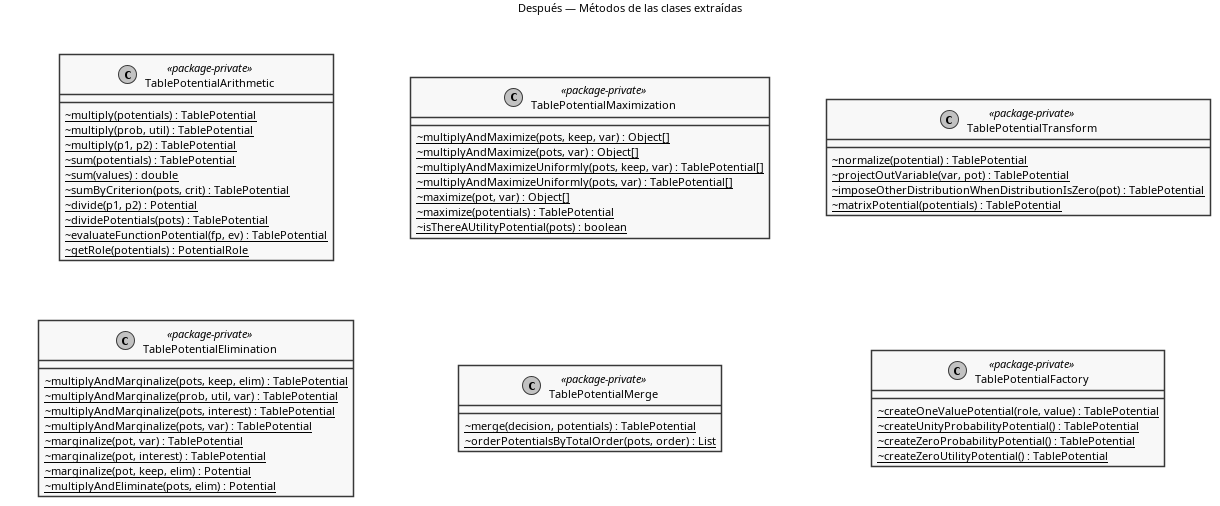
\includegraphics[width=\textwidth]{despues-detalle}
  \caption{Detalle de los métodos de cada clase extraída: Arithmetic (10 métodos), Elimination (8), Maximization (7), Merge (2), Transform (4), Factory (4).}
  \label{fig:dpo-detalle}
\end{figure}

\subsection{Por qué aporta}

\begin{enumerate}
  \item \textbf{Transparencia total:} Los 28 callers existentes en \texttt{core} e \texttt{inference} no requirieron ningún cambio. El Facade delega exactamente igual que antes.
  \item \textbf{Localización de bugs:} Si hay un bug en la multiplicación de potenciales, solo hay que mirar \texttt{TablePotentialArithmetic} ($\sim$450 líneas), no 2.175 líneas. Los helpers privados están junto a los métodos que los usan.
  \item \textbf{Navegabilidad:} Cada fichero tiene un propósito claro anunciado por su nombre. Un desarrollador nuevo puede entender la estructura en segundos.
  \item \textbf{Paralelización futura:} Las clases concurrentes en \texttt{potential/operation/concurrent/} podrían extender las clases individuales en vez de duplicar la clase monolítica.
\end{enumerate}

%==============================================================================
\section{Rediseño de la jerarquía de potenciales}
\label{sec:potenciales}
%==============================================================================

\noindent\textit{Documento completo:} \texttt{docs/rediseno-potenciales/rediseno-potenciales.tex}

\subsection{Problema}

La jerarquía de potenciales tenía tres defectos estructurales:

\begin{enumerate}
  \item \textcolor{problem}{\textbf{TablePotential sobrecargada:}} Contenía \texttt{strategyTrees[]} y \texttt{uncertainValues[]}, ambos \texttt{null} en la inmensa mayoría de las instancias. Todos los métodos (\texttt{tableProject}, \texttt{reorder}, \texttt{deepCopy}) contenían \textbf{bloques condicionales triples}: ``si tiene strategies haz A, si tiene uncertainty haz B, si no haz C''. Además, el constructor de copia hacía alias mutable compartido (\texttt{uncertainValues = pot.uncertainValues}): modificar la copia corrompía el original.
  \item \textcolor{problem}{\textbf{GTablePotential heredaba de TablePotential:}} Pero no usaba el array \texttt{values[]} --- solo \texttt{elementTable}. Heredar de \texttt{TablePotential} reservaba \texttt{tableSize * 8 bytes} de memoria que nunca se utilizaban.
  \item \textcolor{problem}{\textbf{Sin abstracción intermedia:}} Los campos de indexación (\texttt{dimensions[]}, \texttt{offsets[]}, \texttt{tableSize}) eran comunes a ambas familias pero estaban duplicados en \texttt{TablePotential}.
\end{enumerate}

\begin{figure}[H]
  \centering
  
\includegraphics[width=1.0\textwidth]{before}
  \caption{Antes: \texttt{TablePotential} contiene tres responsabilidades mezcladas (values, strategyTrees, uncertainValues). \texttt{GTablePotential} hereda un array \texttt{values[]} que nunca usa, con \texttt{tableSize * 8 bytes} de desperdicio por instancia.}
  \label{fig:pot-antes}
\end{figure}

\subsection{Solución}

Refactorización en 5 fases: extracción de \texttt{AbstractIndexedPotential}, split de \texttt{TablePotential} en 3 clases por el principio de Liskov, y reparentado de \texttt{GTablePotential}.

\begin{figure}[H]
  \centering
  
\includegraphics[width=1.0\textwidth]{after}
  \caption{Después (fases 1--4): \texttt{AbstractIndexedPotential} captura la indexación compartida. \texttt{TablePotential} queda limpia (solo \texttt{values[]}). \texttt{StrategicTablePotential} y \texttt{UncertainTablePotential} encapsulan sus campos específicos. El despacho virtual elimina los bloques condicionales triples.}
  \label{fig:pot-despues}
\end{figure}

\begin{figure}[H]
  \centering
  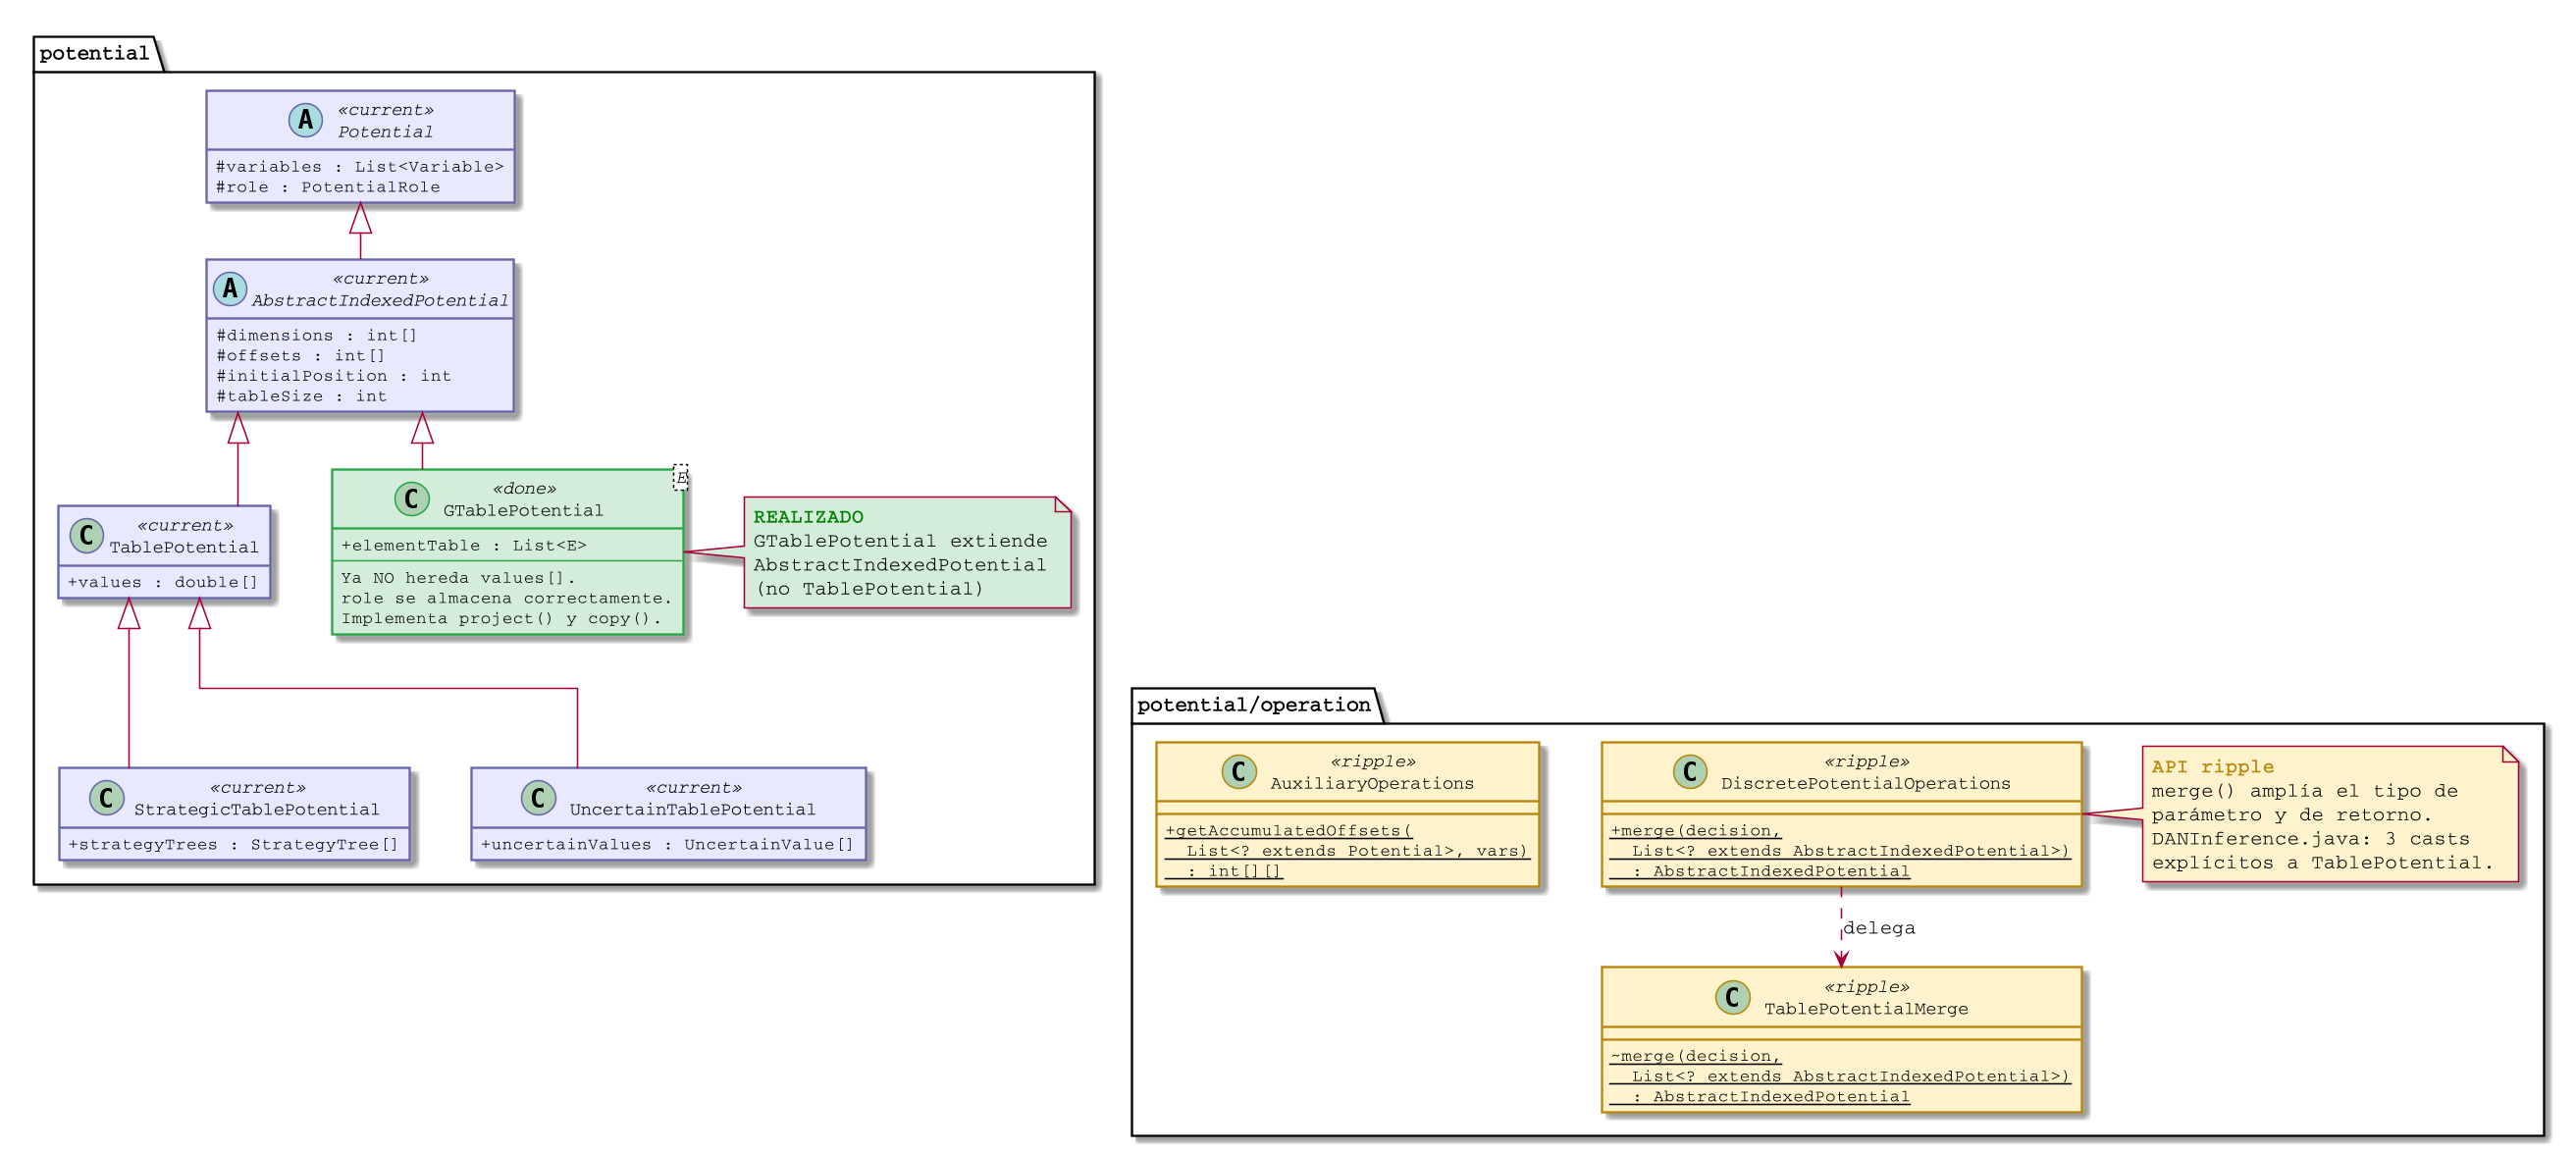
\includegraphics[width=0.85\textwidth]{phase5-implemented}
  \caption{Fase 5 implementada: \texttt{GTablePotential} ahora extiende \texttt{AbstractIndexedPotential} directamente, sin heredar \texttt{values[]}. El \textit{API ripple} en \texttt{merge()} fue contenido: solo 3 casts explícitos en \texttt{DANInference}.}
  \label{fig:pot-phase5}
\end{figure}

\subsection{Por qué aporta}

\begin{enumerate}
  \item \textbf{Principio de sustitución de Liskov:} Antes, \texttt{GTablePotential} violaba LSP: heredaba un contrato (\texttt{values[]} y sus métodos) que no cumplía. Ahora cada clase solo expone lo que realmente implementa.
  \item \textbf{Eliminación de bloques condicionales:} Los triples \texttt{if (strategyTrees != null) ... else if (uncertainValues != null) ... else ...} en \texttt{tableProject()}, \texttt{reorder()}, y \texttt{deepCopy()} se reemplazan por despacho virtual: cada subclase implementa su versión, más simple y verificable.
  \item \textbf{Bug de copia eliminado:} El alias mutable (\texttt{uncertainValues = pot.uncertainValues}) desaparece porque \texttt{UncertainTablePotential.deepCopy()} copia explícitamente su campo. Cada subclase es responsable de su propio deepCopy.
  \item \textbf{Ahorro de memoria:} Cada instancia de \texttt{GTablePotential} (usada en CEA con muchos objetos \texttt{Choice}) ahorra \texttt{tableSize * 8} bytes de arrays \texttt{double[]} no utilizados.
  \item \textbf{Extensibilidad:} Añadir un nuevo tipo de potencial indexado (por ejemplo, \texttt{SparseTablePotential}) solo requiere extender \texttt{AbstractIndexedPotential}, sin modificar \texttt{TablePotential}.
\end{enumerate}

%==============================================================================
\section{Refactorización del sistema de excepciones}
\label{sec:excepciones}
%==============================================================================

\noindent\textit{Documentos:} \texttt{docs/refactorizacion-excepciones-previo/} (análisis) y \texttt{docs/refactorizacion-excepciones-posterior/} (resultado)

\subsection{Problema}

El sistema de excepciones tenía 5 problemas identificados:

\begin{enumerate}
  \item 5 excepciones checked que deberían ser unchecked (el caller no puede recuperarse) contaminaban 53 ficheros con \texttt{throws} clauses innecesarias.
  \item \texttt{SAXException} fugaba desde el parser XML hasta la GUI (\texttt{MainPanelListenerAssistant}), exponiendo detalles de implementación.
  \item \texttt{NonProjectablePotentialException} era una clase plana con 8 causas distintas sin diferenciar --- imposible hacer \texttt{catch} específico.
  \item 34 bloques \texttt{try/catch} repetitivos en \texttt{actionPerformed()}.
  \item Excepciones inalcanzables: \texttt{ThereIsNoNextEvidenceCaseException} nunca se lanzaba porque los botones se deshabilitaban preventivamente.
\end{enumerate}

\begin{figure}[H]
  \centering
  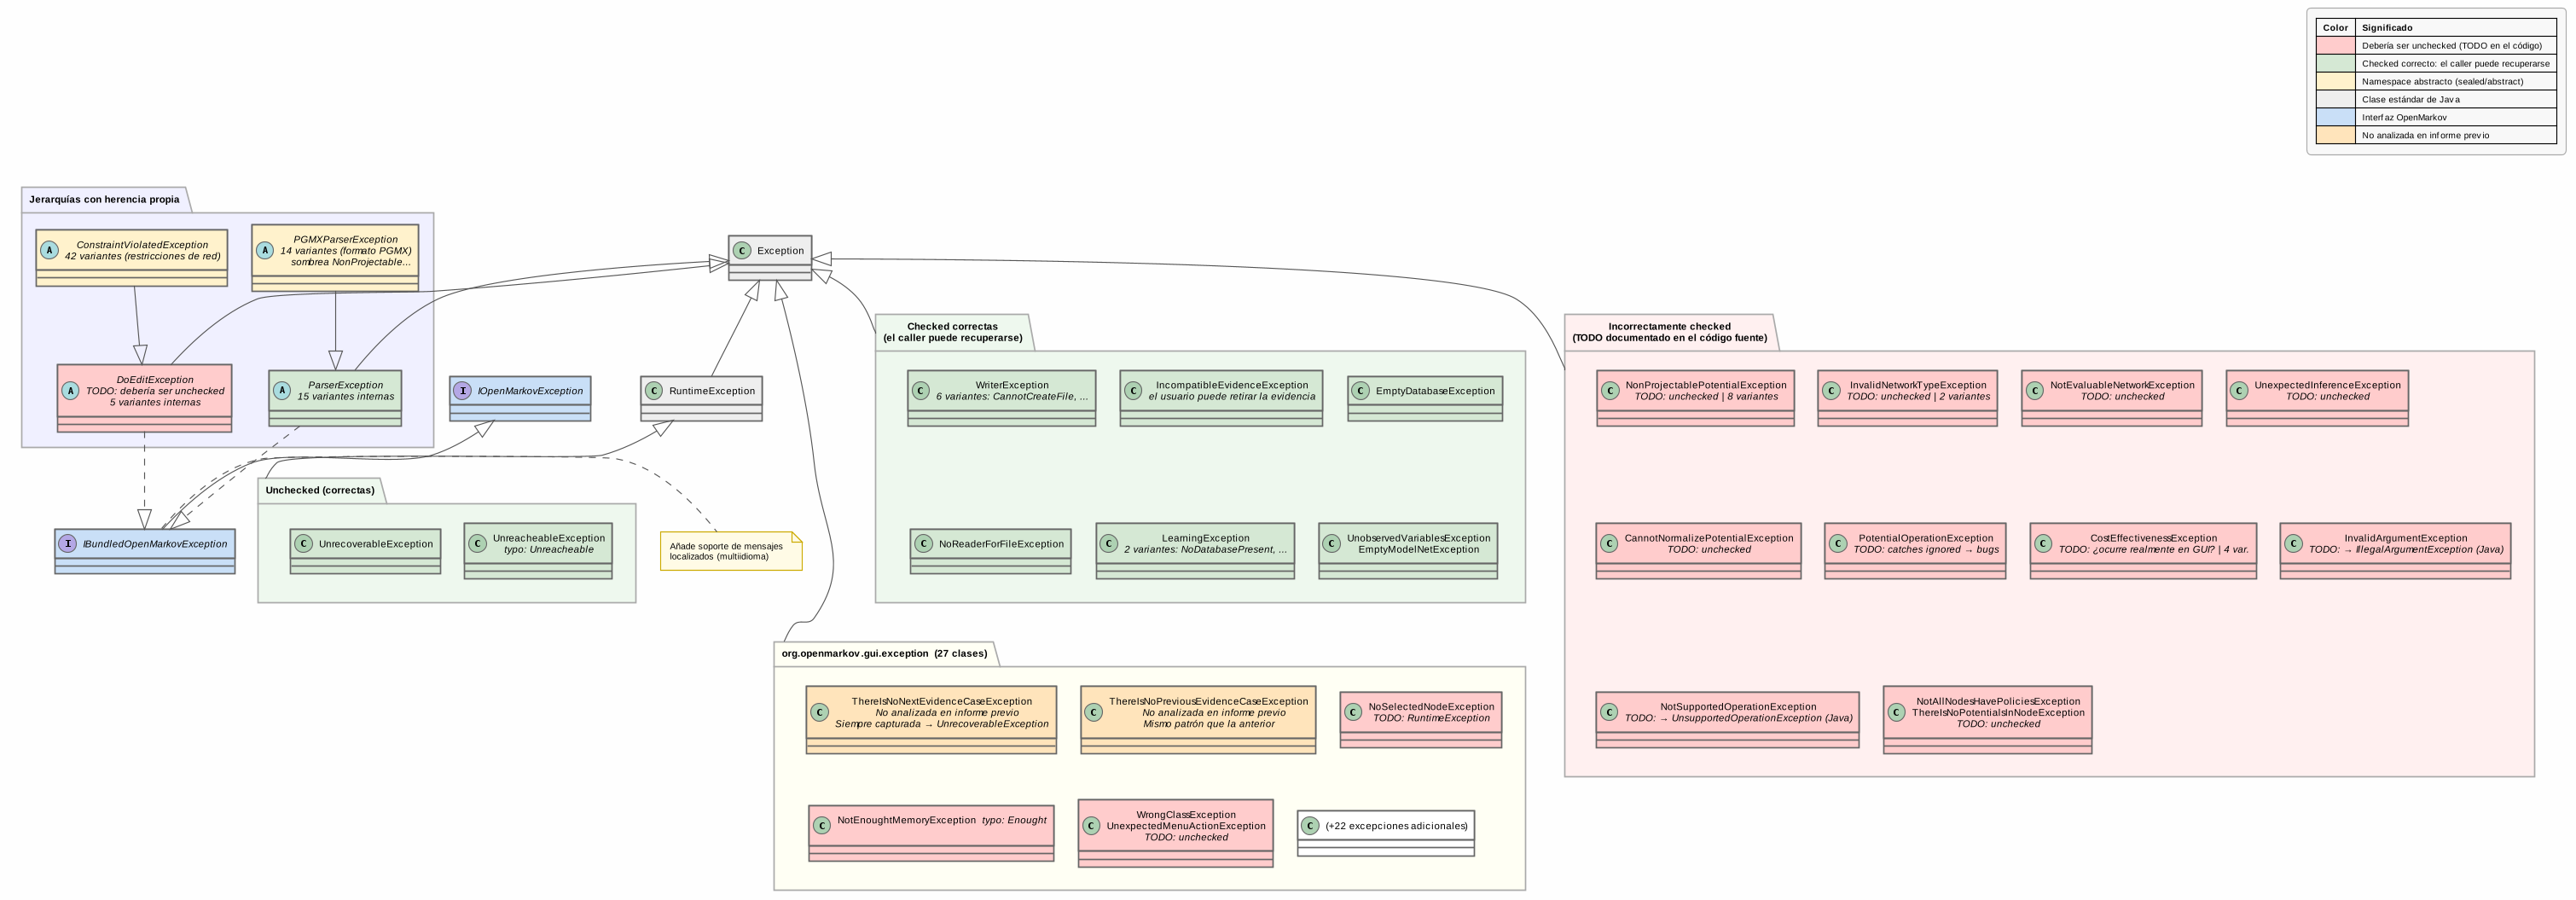
\includegraphics[width=\textwidth]{exception-hierarchy-current}
  \caption{Estado original del sistema de excepciones. Rojo: excepciones incorrectamente checked (marcadas con TODO en el código). Verde: checked correctas. Amarillo: namespaces abstractos. Naranja: no analizadas en informe previo.}
  \label{fig:exc-antes}
\end{figure}

\subsection{Solución}

\begin{figure}[H]
  \centering
  \begin{subfigure}[b]{0.48\textwidth}
    \centering
    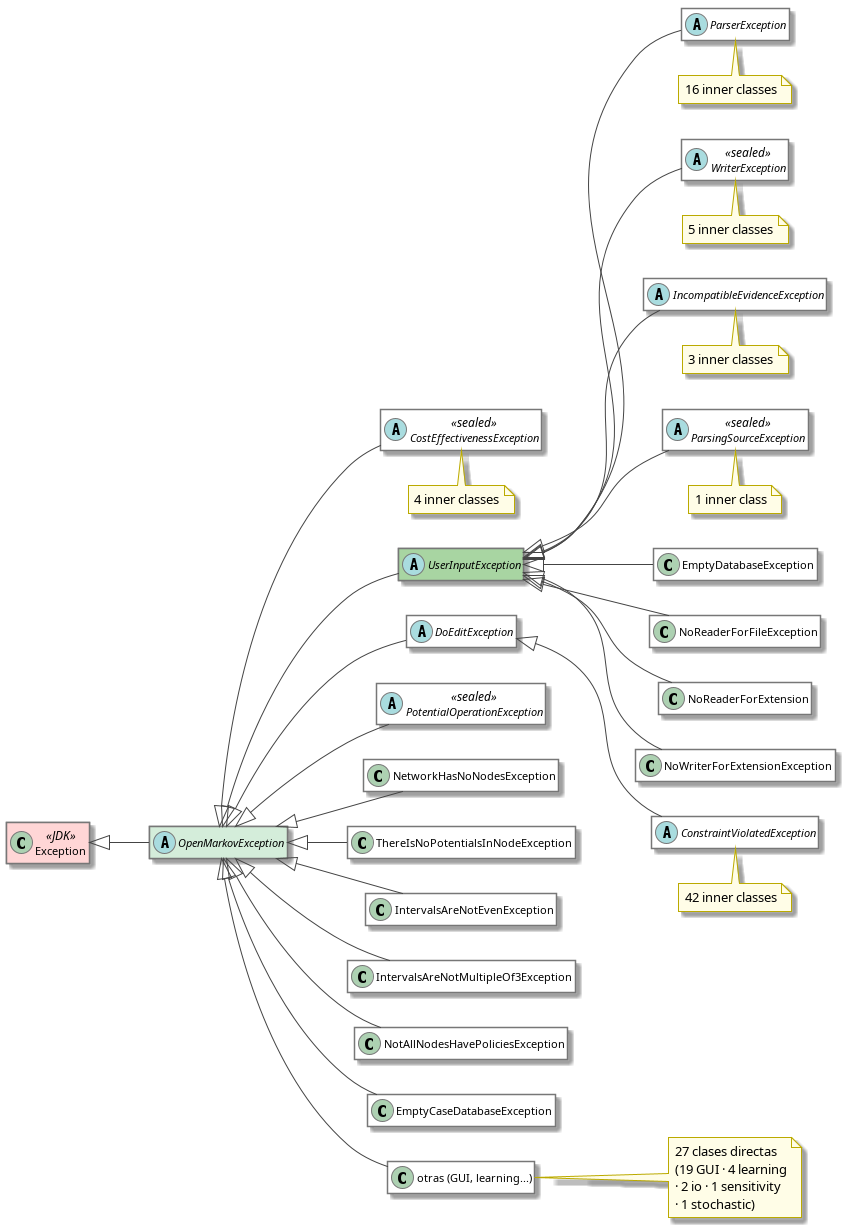
\includegraphics[width=\textwidth]{hierarchy_checked}
    \caption{Jerarquía checked final: \texttt{OpenMarkovException} como base, \texttt{UserInputException} para errores del usuario, \texttt{DoEditException} para fallos en edits.}
    \label{fig:exc-checked}
  \end{subfigure}
  \hfill
  \begin{subfigure}[b]{0.48\textwidth}
    \centering
    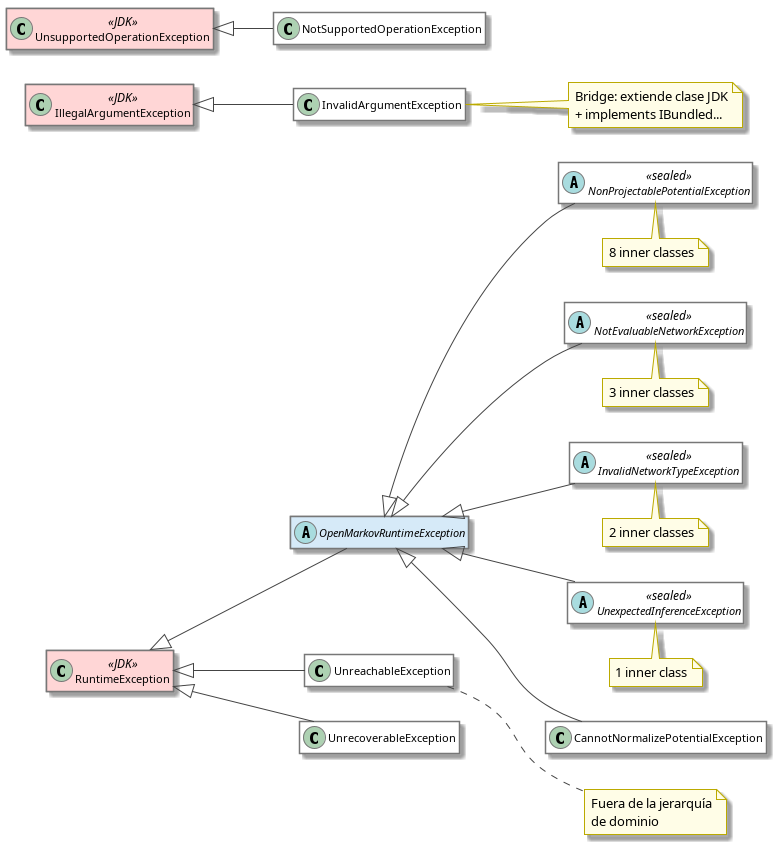
\includegraphics[width=\textwidth]{hierarchy_unchecked}
    \caption{Jerarquía unchecked: \texttt{OpenMarkovRuntimeException} con 4 familias sealed. \texttt{UnreachableException} fuera de la jerarquía de dominio.}
    \label{fig:exc-unchecked}
  \end{subfigure}
  \caption{Sistema de excepciones después de la refactorización.}
\end{figure}

\begin{figure}[H]
  \centering
  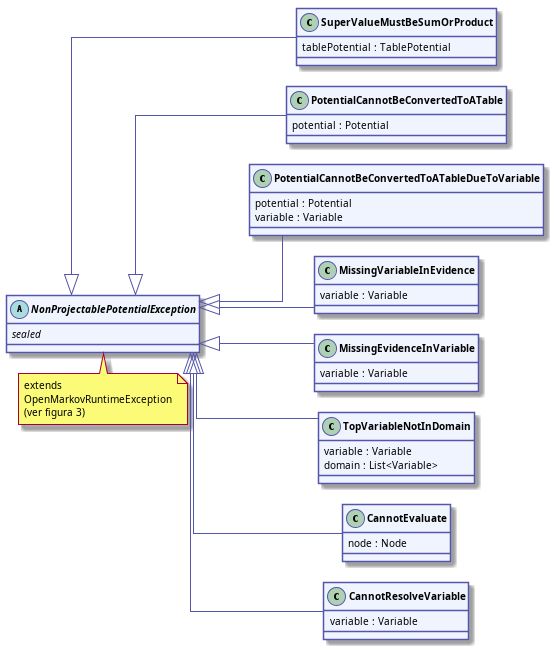
\includegraphics[width=0.7\textwidth]{nonprojectable_hierarchy}
  \caption{\texttt{NonProjectablePotentialException} como clase \texttt{sealed} con 8 subtipos semánticos. Cada subtipo lleva la información contextual necesaria (el potencial, la variable, el nodo) para un diagnóstico preciso.}
  \label{fig:exc-nonproj}
\end{figure}

\subsection{Por qué aporta}

\begin{enumerate}
  \item \textbf{Limpieza de throws:} 40 cláusulas \texttt{throws} eliminadas en 53 ficheros. Cada método de inferencia ya no obliga a sus callers a manejar excepciones de las que no pueden recuperarse.
  \item \textbf{Encapsulación:} La \texttt{SAXException} ya no llega a la GUI; el parser la envuelve en \texttt{ParserException}. Si mañana se cambia JDOM2 por StAX, la GUI no se ve afectada.
  \item \textbf{Diagnóstico preciso:} Con la sealed hierarchy, un \texttt{catch (NonProjectablePotentialException e)} puede hacer \texttt{switch} para distinguir las 8 causas. Antes, el mensaje de error era siempre genérico.
  \item \textbf{Sealed classes (Java 17):} El compilador garantiza que el \texttt{switch} sobre los subtipos es exhaustivo. Si se añade un 9.º subtipo, todos los switches se marcan como incompletos en compilación.
\end{enumerate}

%==============================================================================
\section{Heurísticas de eliminación de variables}
\label{sec:heuristicas}
%==============================================================================

\noindent\textit{Documento completo:} \texttt{docs/heuristic/heuristicas.tex}

Se corrigieron 2 bugs en \texttt{CanoMoralElimination} y se añadieron 4 nuevas heurísticas (1 greedy + 3 lookahead):

\begin{figure}[H]
  \centering
  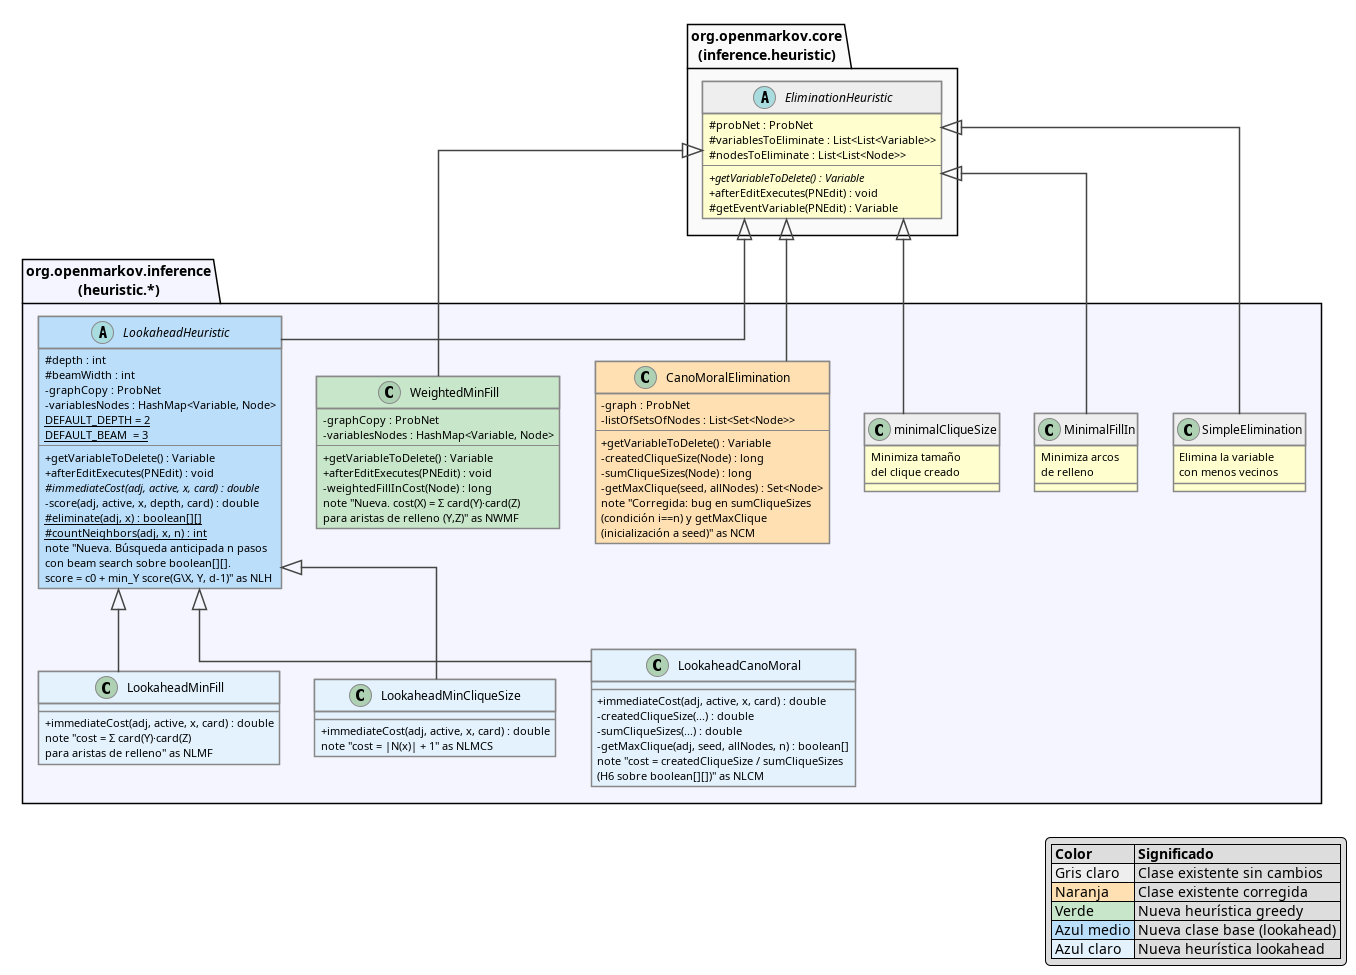
\includegraphics[width=\textwidth]{diagrama_clases}
  \caption{Heurísticas de eliminación. Naranja: \texttt{CanoMoralElimination} corregida (bug en \texttt{sumCliqueSizes} y en \texttt{getMaxClique}). Verde: \texttt{WeightedMinFill} (nueva greedy). Azul: framework \texttt{LookaheadHeuristic} con 3 implementaciones que miran $n$ pasos adelante con beam search.}
  \label{fig:heuristicas}
\end{figure}

\subsection{Por qué aporta}

\begin{enumerate}
  \item \textbf{Bug en CanoMoral:} \texttt{sumCliqueSizes()} siempre devolvía 0 (condición \texttt{i < numMaximalCliques} en vez de \texttt{i == numMaximalCliques}), haciendo que la heurística usara solo \texttt{createdCliqueSize} sin su divisor. El segundo bug (\texttt{getMaxClique} inicializado a \texttt{null}) causaba NPE cuando el clique semilla era el máximo.
  \item \textbf{WeightedMinFill:} Supera a \texttt{MinimalFillIn} en redes donde los nodos tienen cardinalidades muy dispares (frecuente en redes médicas), porque pondera el relleno por el producto de cardinalidades en vez de contar solo aristas.
  \item \textbf{Lookahead:} En la red \texttt{BN-hepar} (70 nodos), \texttt{LookaheadMinFill} reduce el coste del árbol de unión de 713 a 628 (--12\%) respecto a \texttt{MinimalFillIn}, a cambio de un tiempo de compilación aceptable gracias al beam search.
\end{enumerate}

%==============================================================================
\section{Corrección de bugs}
%==============================================================================

\begin{longtable}{p{1.2cm}p{5cm}p{6.5cm}}
\toprule
\textbf{Issue} & \textbf{Descripción} & \textbf{Solución} \\
\midrule
\endfirsthead
\toprule
\textbf{Issue} & \textbf{Descripción} & \textbf{Solución} \\
\midrule
\endhead
\#456 & Error al abrir propiedades de nodo con potencial Weibull Hazard & Fix en GUI del diálogo de propiedades de nodo \\
\#472 & \texttt{InvertLinkAndUpdatePotentialsEdit.redo()} asignaba potencial hijo al nodo incorrecto & Corrección de la asignación en \texttt{redo()}. Además, el \texttt{PotentialRole} heredado podía ser \texttt{JOINT\_PROBABILITY} en vez de \texttt{CONDITIONAL\_PROBABILITY} \\
\#486 & Error al evaluar DAN con 2 nodos de utilidad & Fix en inferencia DAN y test de integración \\
\#496 & Valores de coste/efectividad ausentes en árboles de decisión CEA & Fix en generación de árboles de decisión CE \\
\#497 & Árbol de estrategia mostraba \texttt{toString()} verbose & Fix en \texttt{toString()} de nodos de estrategia \\
\#504/\#532 & Redondeo inconsistente en resultados de CEA & Fix en inference + costEffectiveness \\
\#506 & Absorción de nodo decisión permitida con padres desconocidos para el decisor & Verificación de predecesor informacional en \texttt{AbsorbNodeValidator} \\
\#520 & Error al evaluar red con nodo utilidad SumPotential & Fix en evaluación y test de integración \\
\#562 & \texttt{reorder()} devolvía \texttt{null} para AugmentedProbTable & Implementación de \texttt{reorder()} en 12 subclases de Potential \\
--- & PC Algorithm: \texttt{evaluateSeparationSets} filtraba durante descubrimiento & Filtro movido a visualización \\
--- & \texttt{multiply} devolvía \texttt{null} para lista vacía & Fix del caso borde \\
\bottomrule
\end{longtable}

%==============================================================================
\section{Calidad de código transversal}
%==============================================================================

Cambios aplicados simultáneamente a todos los módulos (propagados el 2--3 de abril):

\begin{itemize}
  \item \textbf{470 variables marcadas \texttt{final}} (13 módulos).
  \item \textbf{178 imports no usados eliminados} (12 módulos).
  \item \textbf{502 tags Javadoc añadidos} (\texttt{@param}, \texttt{@return}, \texttt{@throws}) en 14 módulos.
  \item \textbf{Autoría actualizada:} Tag \texttt{@author marias} $\rightarrow$ \texttt{Manuel Arias}.
  \item \textbf{5 PNConstraint subclasses adaptadas} a la nueva API tras extracción de \texttt{GraphNetwork} --- propagado a todos los módulos.
  \item \textbf{Log level corregido:} root logger cambiado de \texttt{TRACE} a \texttt{INFO}.
  \item \textbf{PGMXReader\_0\_2:} Dispatch basado en reflexión reemplazado por interfaz funcional tipada.
  \item \textbf{hasValidStructure/isValidNode:} Corregidos --- antes devolvían siempre \texttt{true}.
\end{itemize}

%==============================================================================
\section{Tests nuevos}
%==============================================================================

\begin{itemize}
  \item \textbf{core --- Invariantes algebraicos:} \texttt{DiscretePotentialOperationsAlgebraicInvariantsTest} --- marginales suman 1, normalize preserva estructura, multiply asociativa.
  \item \textbf{core --- Regresión tableProject:} Todos los patrones de proyección cubiertos.
  \item \textbf{core --- Tests unitarios:} \texttt{CriterionTest}, \texttt{FindingTest}, \texttt{TablePotentialArithmeticEdgeCasesTest}.
  \item \textbf{core --- Pre-reparenting:} Coverage de \texttt{GTablePotential}, \texttt{Choice} y flujos CEA antes del reparentado.
  \item \textbf{integrationtests --- Invariantes de probabilidad:} Verifica invariantes para \textbf{todas} las variables de cada BN.
  \item \textbf{integrationtests --- PGMXReadersTest:} Adaptado para 8 tipos de potencial sin parsers directos.
  \item \textbf{integrationtests --- Issues:} Tests de regresión para \#486 y \#520.
\end{itemize}

%==============================================================================
\section{Resumen de métricas}
%==============================================================================

\begin{center}
\begin{tabular}{lr}
\toprule
\textbf{Métrica} & \textbf{Valor} \\
\midrule
Commits totales (10 días) & 152 \\
Módulos afectados & 19 de 21 \\
Bugs corregidos (issues) & 11 \\
Variables marcadas \texttt{final} & $\sim$470 \\
Imports eliminados & 178 \\
Tags Javadoc añadidos & 502 \\
Clases extraídas (Extract Class) & 12 \\
Clases nuevas de test & $\sim$10 \\
Tests nuevos & $\sim$100+ \\
Diagramas UML (PlantUML) & 51 \\
Documentos técnicos (LaTeX) & 12 \\
\bottomrule
\end{tabular}
\end{center}

%==============================================================================
\section{Trabajo pendiente}
%==============================================================================

\begin{enumerate}
  \item \textbf{ProbNet --- fases 5--6:} Evaluar extracción de \texttt{reader}/\texttt{writer} (alto riesgo, pendiente).
  \item \textbf{Tests de ProbNet:} Llevar cobertura al objetivo $>$80\%. Gaps críticos: clasificación, agentes, I/O, metadatos.
  \item \textbf{Edits concretos:} 55 edits con solo 1 fichero de test. Cada edit debería tener tests propios.
  \item \textbf{EM Algorithm:} Sigue deshabilitado. Pendiente de decisión sobre su futuro.
  \item \textbf{Candidatos a diagramas UML (23):} Identificados en la auditoría de Javadoc pero aún sin implementar la mayoría.
\end{enumerate}

\end{document}
